\documentclass[10pt,a4paper]{report}
\usepackage[utf8]{inputenc}
\usepackage{amsmath}
\usepackage{amsfonts}
\usepackage{amssymb}
\usepackage{graphicx}
\usepackage{caption}
\usepackage{subcaption}
\usepackage{listings}
\usepackage{url}


\author{Huaiyu Du, Cairong Yang, Athmar Shamhan}
\begin{document}
\title{Face Mask Detection}

\maketitle

\chapter{Task Description}
Our goal is to develop an program for mask detection. Given an image, our program would generate an image with ROIs that denote the location of human faces with confidence and labels, including: With mask; Without mask; Mask is worn incorrectly.

\chapter{Dataset}
The chosen dataset "Face Mask Detection" \cite{facemd} is from Kaggle. The dataset consists of 853 human pictures (of different ages and races ) with various illumination and poses. Also, ground truth is provided. Three classes are included in the dataset: With mask; Without mask; Mask is worn incorrectly. However, some faces are masked by hand instead of using masks. Some samples of the chosen dataset are shown in Figure \ref{fig:Samples}.
\begin{figure}[hbtp]
     \centering
     \begin{subfigure}[b]{0.45\textwidth}
         \centering
         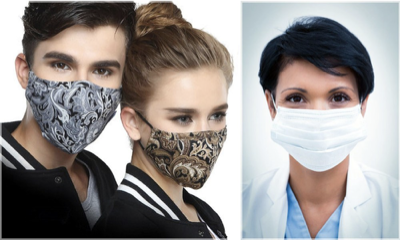
\includegraphics[width=\textwidth]{./imgs/maksssksksss81.png}
         \caption{sample 1}
         \label{fig:Oringial image}
     \end{subfigure}
     \hfill
     \begin{subfigure}[b]{0.45\textwidth}
         \centering
         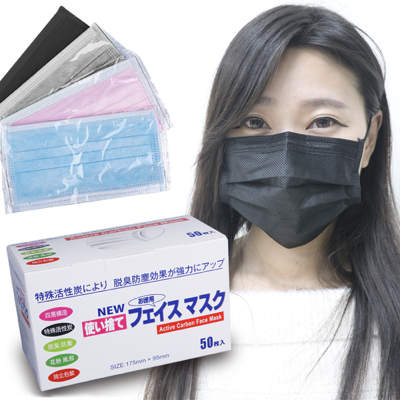
\includegraphics[width=\textwidth]{./imgs/maksssksksss109.png}
         \caption{sample 2}
         \label{fig:Gray scale image}
     \end{subfigure}
     \hfill
     \begin{subfigure}[b]{0.45\textwidth}
         \centering
         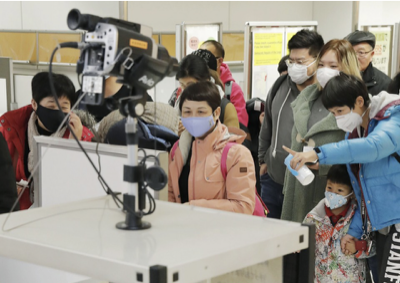
\includegraphics[width=\textwidth]{./imgs/maksssksksss149.png}
         \caption{sample 3}
         \label{fig:Gaussian blur image}
     \end{subfigure}
           \hfill
           \begin{subfigure}[b]{0.45\textwidth}
         \centering
         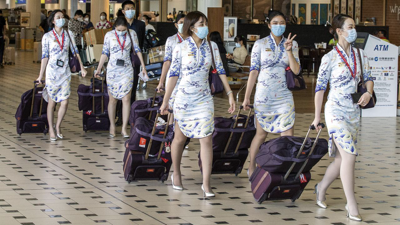
\includegraphics[width=\textwidth]{./imgs/maksssksksss752.png}
         \caption{sample 4}
         \label{fig:Gaussian blur image}
     \end{subfigure}
        \caption{Samples}
        \label{fig:Samples}
\end{figure}

\chapter{Methdology}
\section{over view}
The following Figure \ref{fig:Basic Structure} shows the basic structure of our program. The core of this methodology is the classification network. We need to train a classification network to distinguish four classes: background, with mask, without the mask, mask worn incorrectly. To train the network, we need to cut images based on the dataset labels(ground truth ROI), plus random cuts background images to make our dataset. After the classification network is trained, we can detect face masks for a given image. Firstly, we will use different size sliding windows to cut sub-images from the original image, then feed them to the Classification Network to get the result. Such a result would contain many overlapping RIOs, then use non-maximum suppression method to produce our final result.
\begin{figure}[hbtp]

\centering
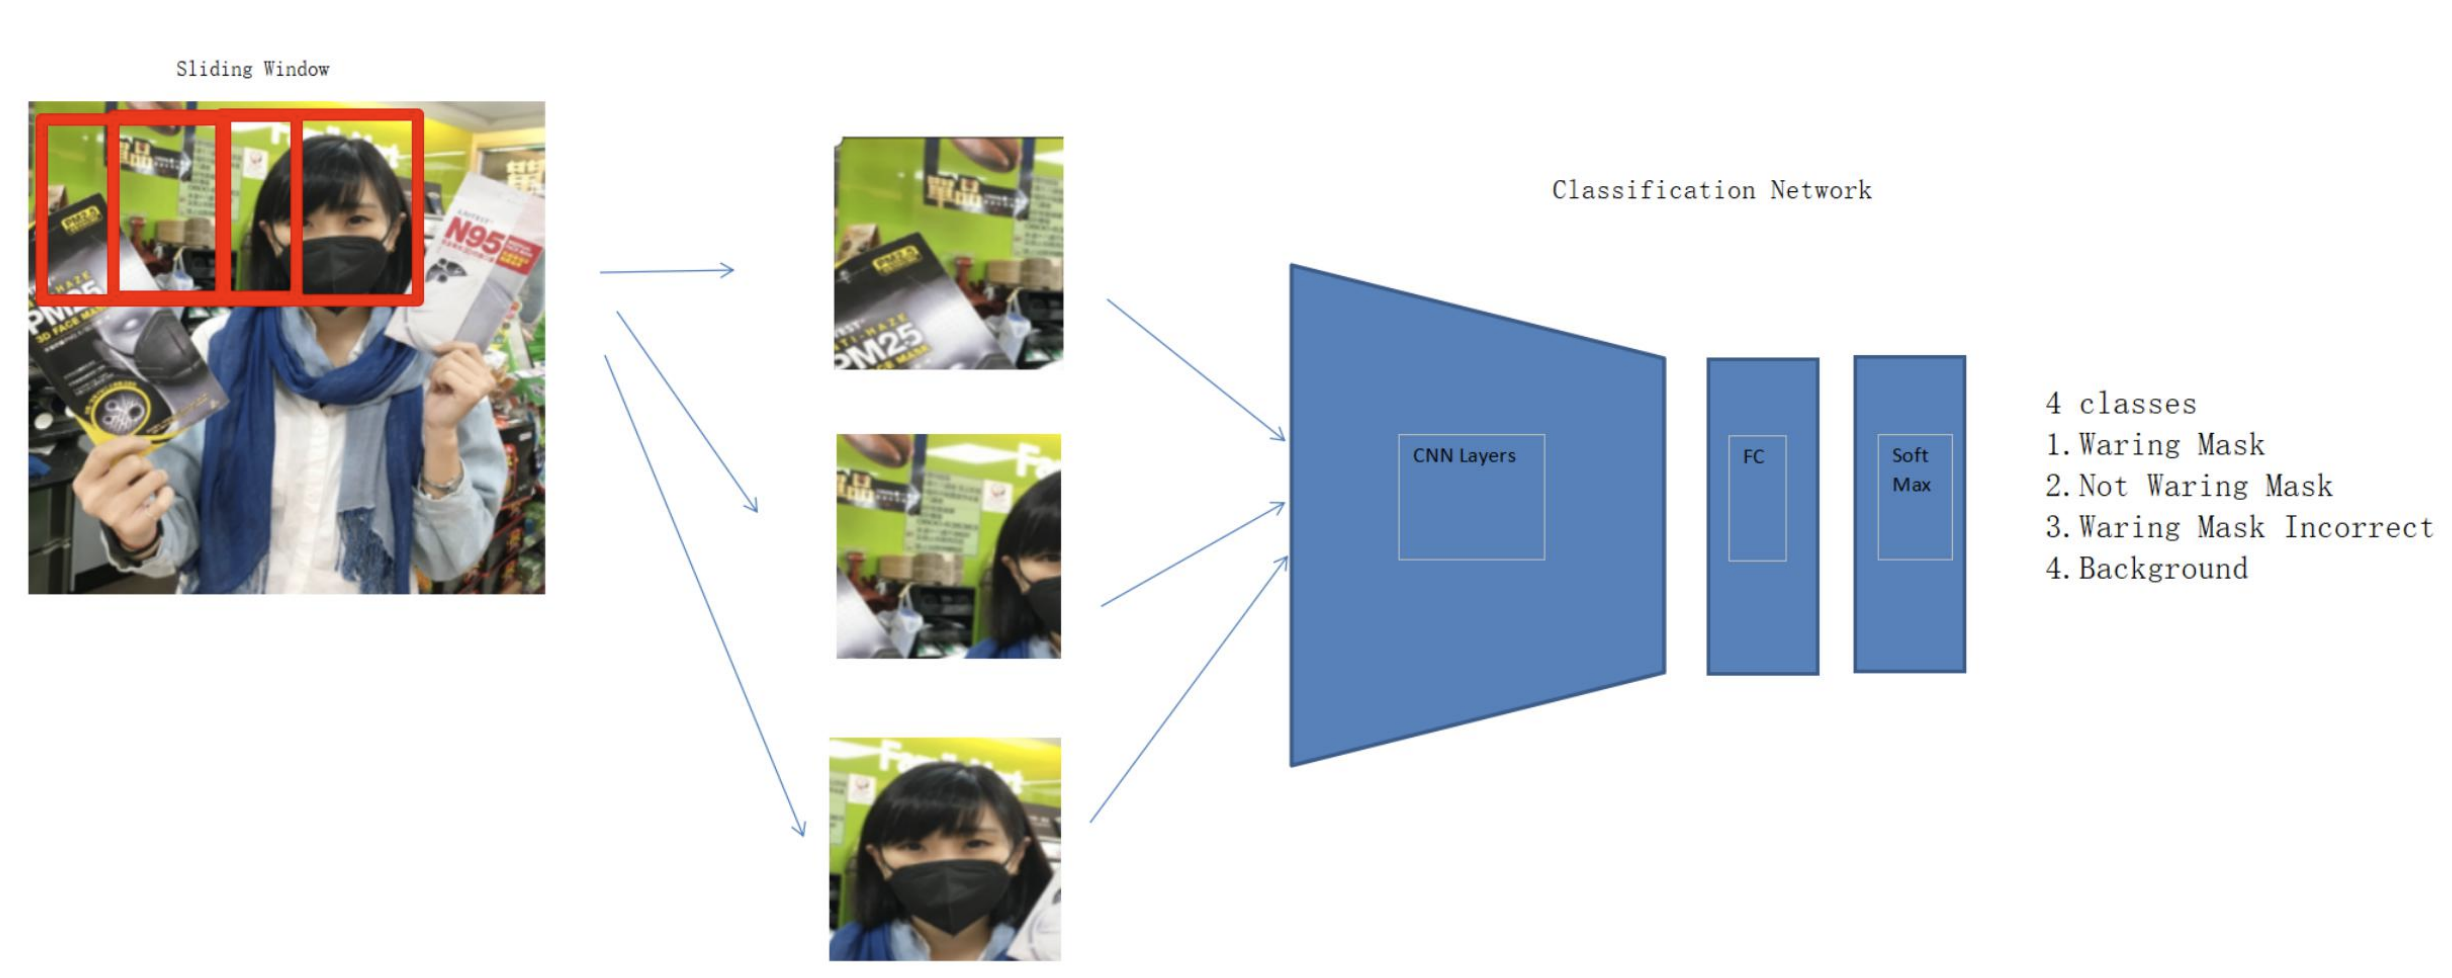
\includegraphics[scale=0.14]{imgs/workflow.png}
\caption{basic structure}
        \label{fig:Basic Structure}
\end{figure}

\section{training data preparation}
\subsection{Dataset analysis}
Kaggle dataset "Face mask detection" consists of 852 images. Each image contains one or more human faces. Ground truth provided as XML files with absolute location and label name. \\
Ground truth annotation sample:
\begin{lstlisting}
<annotation>
	<folder>images</folder>
	<filename>maksssksksss0.png</filename>
	<size>
		<width>512</width>
		<height>366</height>
		<depth>3</depth>
	</size>
	<segmented>0</segmented>
	<object>
		<name>without_mask</name>
		<pose>Unspecified</pose>
		<truncated>0</truncated>
		<occluded>0</occluded>
		<difficult>0</difficult>
		<bndbox>
			<xmin>79</xmin>
			<ymin>105</ymin>
			<xmax>109</xmax>
			<ymax>142</ymax>
		</bndbox>
	</object>
	...
</annotation>
\end{lstlisting}
While, as Figure \ref{fig:Instance numbers} shown. the instance number of each class is quite unbalanced. With mask class has 3232 instances, without mask class has 717 instances while the mask wore incorrectly class only has 123 instances. 
\subsection{Dataset preparation}
We wrote a program to chop the sub-images according to the ground truth to prepare the classification training dataset. To make our classification network training dataset more balanced, we have to use image processing approaches such as random rotation and flipping to generate more images for categories "without the mask" and "mask worn incorrectly". We randomly chop 20 images of different sizes and less than 0.2 UOI with ground truth from each image as a background class dataset. There are 852 images in total; chopped images are divided into three categories according to original images' indices. \\
Training set: from 1 to 600. \\
Validation set: from 601 to 750. \\
Test set: from 751 to 852.  
\begin{figure}[hbtp]

\centering
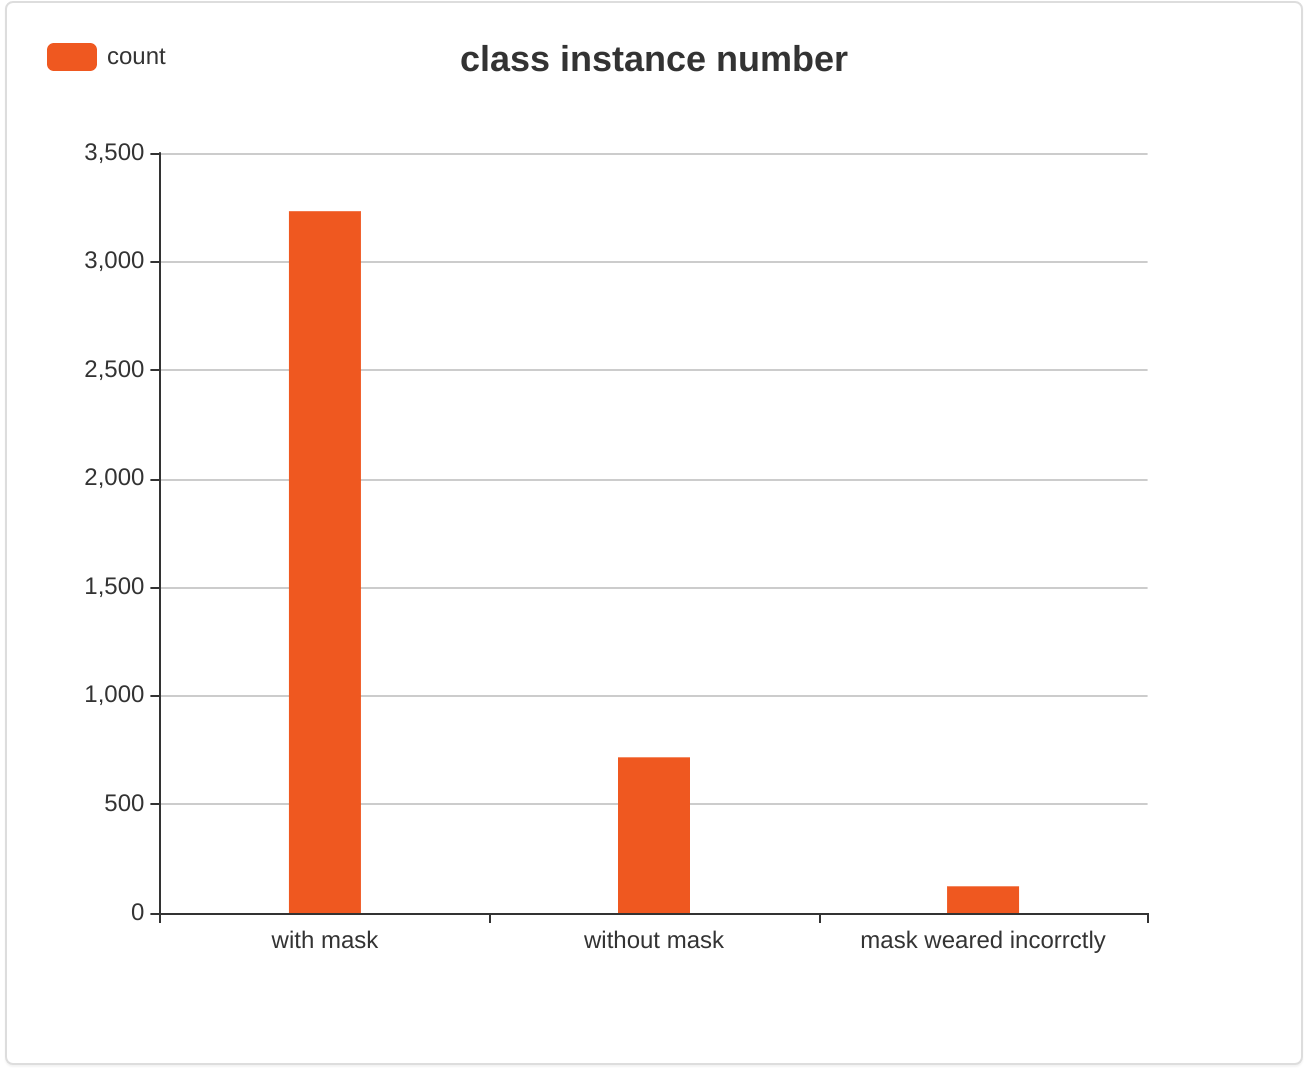
\includegraphics[scale=0.2]{imgs/instance numbers.png}
\caption{Instance numbers}
        \label{fig:Instance numbers}
\end{figure}

\section{classification model}
Here we use the PyTorch framework to make our classification network. Our first version is quite simple. It takes a 24 * 24 image as input, only has two convolutional layers and one fully-connected layer. Such a network's performance is relatively poor. On the one hand, we do not have enough data to train a high-accuracy network. On the other hand, the network structure is too simple.\\
So we decide to use transfer learning to obtain a high accuracy classification network. Form PyTorch framework, we downloaded the pre-trained VGG16 model and redefined the classification layers suitable for four classes. All feature extraction layers are frozen. We train the network on our training dataset and validate it on the validation set. After 50 epochs training, save the model which has the best accuracy on the validation set.
\section{main function}
Firstly, we predefined different sizes (from 24 * 24 to 200 * 200) of windows and strides. Using such windows and strides, go through the input image and chop a set of sub-images. Meanwhile, record the absolute locations of each image. Then feed all these sub-images to our classification model. After getting the results, get rid of records that belong to "background", then use the non-maximum suppression method to eliminate the overlapping ROIs. Finally, we can output an image with ROIs and class labels.  
\section{traning process}
Although the method is not complicated, we took our several rounds to fine turn the whole program.
\subsection{First Round}
As mentioned, our first classification network is quite simple and not well trained; the final result is a failure. As Figure \ref{fig:f1} shown, the result is not make sense.
 \begin{figure}[hbtp]

\centering
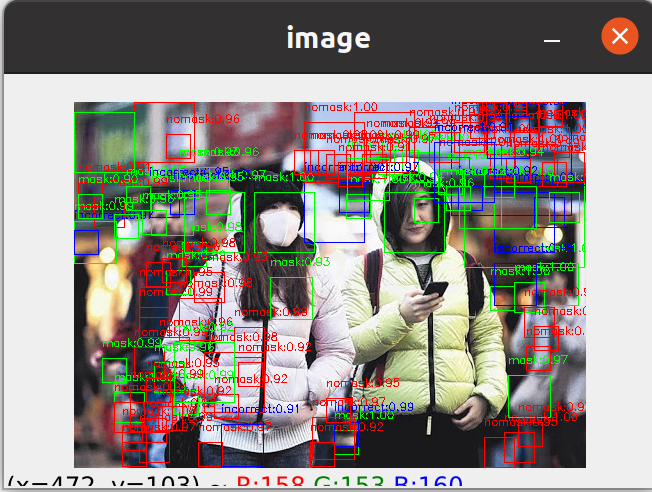
\includegraphics[scale=0.4]{imgs/r1.png}
\caption{First round result sample}
        \label{fig:f1}
\end{figure}

\subsection{Second Round}
Then we use a pre-trained VGG16 model for transfer learning. After 50 epochs training, the accuracy on the validation set is over 90 percent. As Figure \ref{fig:f2} shows, the result somehow makes sense but is still not good enough.
\begin{figure}[hbtp]

\centering
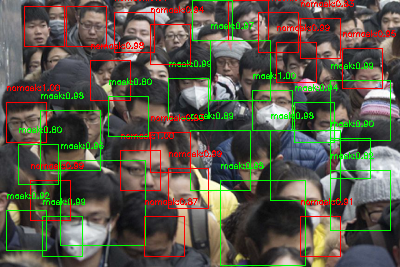
\includegraphics[scale=1.5]{imgs/r2.png}
\caption{Second round result sample}
        \label{fig:f2}
\end{figure}

\subsection{Thrid Round}
We expanded our training set with another dataset on Kaggle "Face Mask Detection ~12K Images Dataset" \cite{face12k} to make our classification model performs better. This dataset only contains facial images with/without masks, which is quite similar to the chopped images produced by ourselves. Furthermore, we unfroze the last four convolutional layers as well. After 50 epochs of training, the accuracy on the validation set is over 97 percent. As Figure \ref{fig:f3} shows, the True Positive prediction is much better. But there are lots of False Positive predictions. The reason is that background is chopped randomly, but in practice, some background might look similar to the positive samples in our training set, and our model can not distinguish them.
\begin{figure}[hbtp]
     \centering
     \begin{subfigure}[b]{0.8\textwidth}
         \centering
         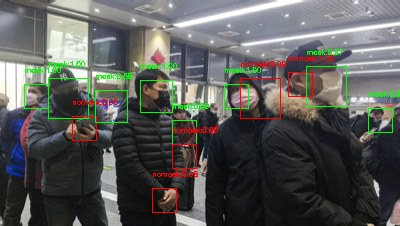
\includegraphics[width=\textwidth]{./imgs/r31.png}
         \caption{sample 1}
         \label{fig:Thrid round sample 1}
     \end{subfigure}
     \hfill
     \begin{subfigure}[b]{0.6\textwidth}
         \centering
         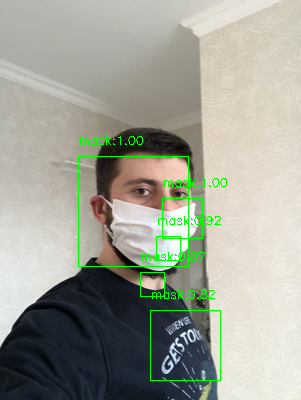
\includegraphics[width=\textwidth]{./imgs/r32.png}
         \caption{sample 2}
         \label{fig:Thrid round sample 2}
     \end{subfigure}

        \caption{Thrid Round Samples}
        \label{fig:f3}
\end{figure}
\subsection{Forth Round}
We collect all the False Positive samples from images 1 to 750 and add them to the background class of training and validation set. Then train our network with the last four convolutional layers and classification layers unfrozen. After 25 epochs, the validation accuracy is over 97 percent. And as Figure \ref{fig:f4} shows, the result seems much better.
 \begin{figure}[hbtp]

\centering
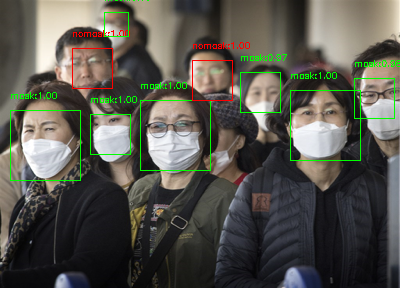
\includegraphics[scale=0.8]{imgs/r4.png}
\caption{Forth round result sample}
        \label{fig:f4}
\end{figure}



\chapter{Evaluation}
We choose Average Precision (AP), Precision and Recall curve as object detection metrics. The following evaluate results and figures are generated via an open-source tool \cite{odm}. The threshold of IOU is set to 0.5. We evaluate our method on images from 751 to 852, which never touched during our training process.
As Figure \ref{fig:e} shows, the "with mask" class has the best accuracy, which AP is 73.35\%, and the "without mask" class's AP is 43.65\%. Not surprisingly "Wore Mask Incorrectly" class has the worst AP value, only 15.71\%, since we do not have enough data for this class.
\begin{figure}[hbtp]
     \centering
     \begin{subfigure}[b]{0.8\textwidth}
         \centering
         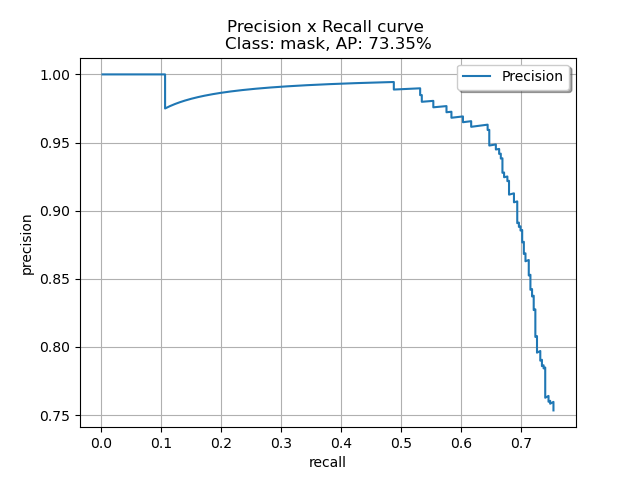
\includegraphics[width=\textwidth]{./imgs/mask.png}
         \caption{With Mask}

     \end{subfigure}
     \hfill
     \begin{subfigure}[b]{0.8\textwidth}
         \centering
         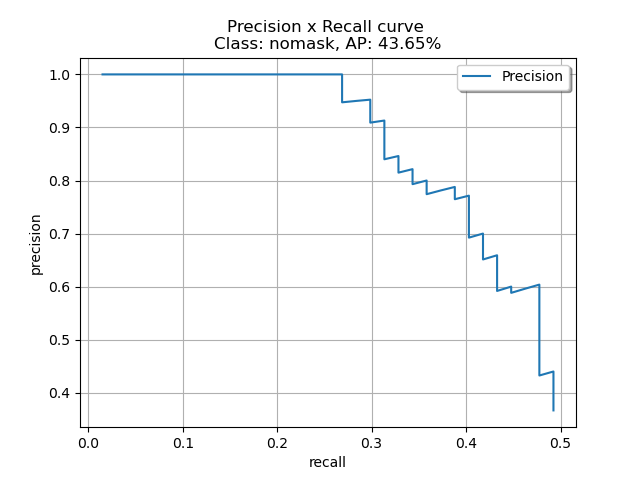
\includegraphics[width=\textwidth]{./imgs/nomask.png}
         \caption{Without Mask}
     \end{subfigure}
          \hfill
     \begin{subfigure}[b]{0.8\textwidth}
         \centering
         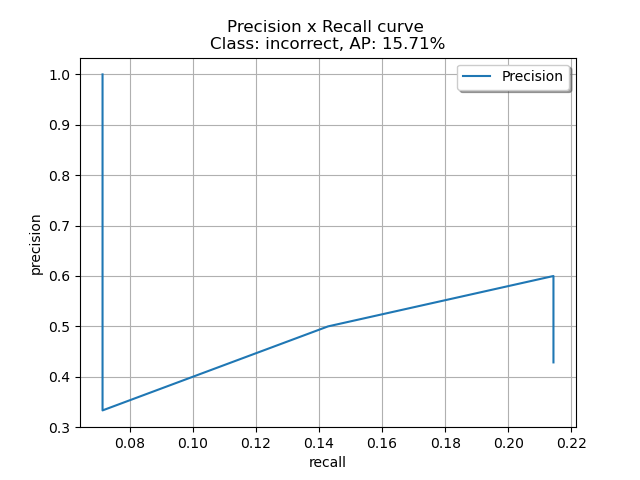
\includegraphics[width=\textwidth]{./imgs/incorrect.png}
         \caption{Wore Mask Incorrectly}
     \end{subfigure}

        \caption{Evaluation Result}
        \label{fig:e}
\end{figure}
\chapter{result samples}

\begin{figure}[hbtp]
     \centering
     \begin{subfigure}[b]{0.45\textwidth}
         \centering
         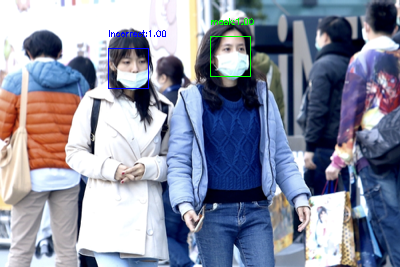
\includegraphics[width=\textwidth]{./imgs/good/maksssksksss756.png}
     \end{subfigure}
     \hfill
     \begin{subfigure}[b]{0.45\textwidth}
         \centering
         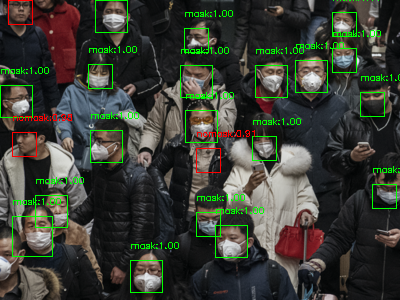
\includegraphics[width=\textwidth]{./imgs/good/maksssksksss795.png}
     \end{subfigure}
     \hfill
     \begin{subfigure}[b]{0.45\textwidth}
         \centering
         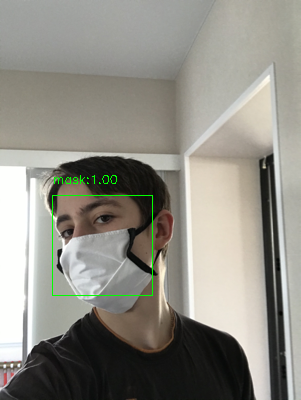
\includegraphics[width=\textwidth]{./imgs/good/maksssksksss765.png}
     \end{subfigure}
               \hfill
     \begin{subfigure}[b]{0.45\textwidth}
         \centering
         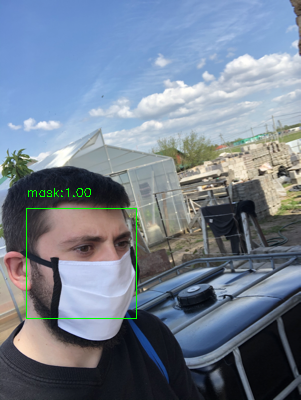
\includegraphics[width=\textwidth]{./imgs/good/maksssksksss764.png}
     \end{subfigure}
\caption{Good samples}
\label{fig:good}
\end{figure}

\begin{figure}[hbtp]
     \centering
     \begin{subfigure}[b]{0.45\textwidth}
         \centering
         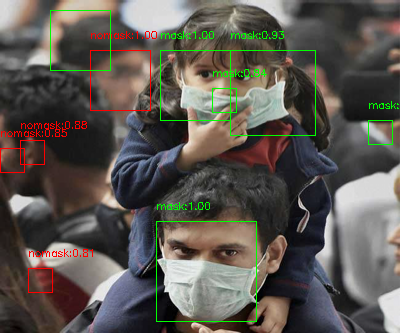
\includegraphics[width=\textwidth]{./imgs/bad/maksssksksss798.png}
     \end{subfigure}
     \hfill
     \begin{subfigure}[b]{0.45\textwidth}
         \centering
         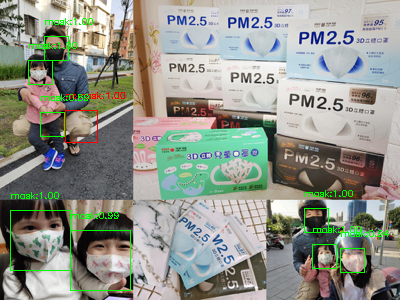
\includegraphics[width=\textwidth]{./imgs/bad/maksssksksss799.png}
     \end{subfigure}
     \hfill
     \begin{subfigure}[b]{0.45\textwidth}
         \centering
         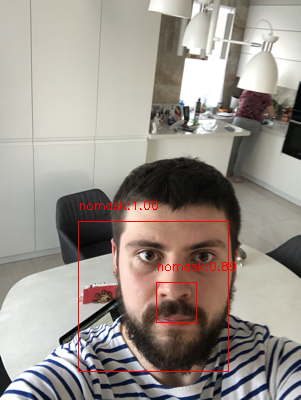
\includegraphics[width=\textwidth]{./imgs/bad/maksssksksss818.png}
     \end{subfigure}
               \hfill
     \begin{subfigure}[b]{0.45\textwidth}
         \centering
         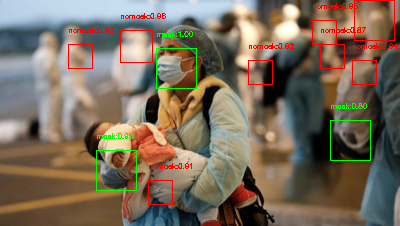
\includegraphics[width=\textwidth]{./imgs/bad/maksssksksss846.png}
     \end{subfigure}
\caption{Bad samples}
\label{fig:good}
\end{figure}
\chapter{Conclusion}
In conclusion, this program can achieve a reasonable accuracy to detect human faces with masks; for worn masks incorrectly, the accuracy is not ideal because of the lack of training samples. We believe that with more samples of the wore masks incorrectly, we can improve the performance of our algorithm.  \\
During the implementation, we also expericence the drawbacks of sliding window approach.
\begin{enumerate}
\item Such an approach can not segment the target objects with high accuracy ROIs because the ROI's size and shape are predefined and can not adjust accordingly. To fits most cases, we define the windows as squires, while the ground truth is not always a square.
\item The Sliding window approach needs lots of computation. To match different size target objects for each image, we need to use different size windows to generate ten thousand sub-images to classify. Even on an RTX3060 GPU, it takes minutes to process one image.

\end{enumerate}

\bibliographystyle{plain}
\bibliography{Reference}
\end{document}